\documentclass[11pt]{report}
\usepackage{tikz}
\usepackage{tkz-graph}
\usepackage{amsmath}
\usepackage{placeins}
\usepackage{caption}
\usepackage{booktabs}
\newcommand\independent{\protect\mathpalette{\protect\independenT}{\perp}}
   \def\independenT#1#2{\mathrel{\rlap{$#1#2$}\mkern4mu{#1#2}}}
\usetikzlibrary{fit,positioning}
\tikzset{
  LabelStyle/.style = { rectangle, rounded corners, draw,
                        minimum width = 2em, fill = yellow!50,
                        text = red, font = \bfseries },
  VertexStyle/.append style = { inner sep=5pt,
                                font = \Large\bfseries},
  EdgeStyle/.append style = {-, bend left} }
\setcounter{chapter}{9}
\begin{document}
\chapter{Problems}
\section{}
\textit{The joint probability model between variables $\{x_i\}_{i=1}^7$ factorizes as}
\begin{equation} 
\begin{aligned}
&Pr(x_1, x_2, x_3, x_4, x_5, x_6, x_7) = \\
&\quad \quad Pr(x_1) Pr(x_3) Pr(x_7) Pr(x_2 | x_1, x_3) Pr(x_5 | x_7, x_2) Pr(x_4 | x_2) Pr (x_6 | x_5, x_4) \notag
\end{aligned}
\end{equation}
\textit{Draw a directed graphical model relating these variables. Which variables form the Markov blanket of variable $x_2$?}
\begin{figure}[h]
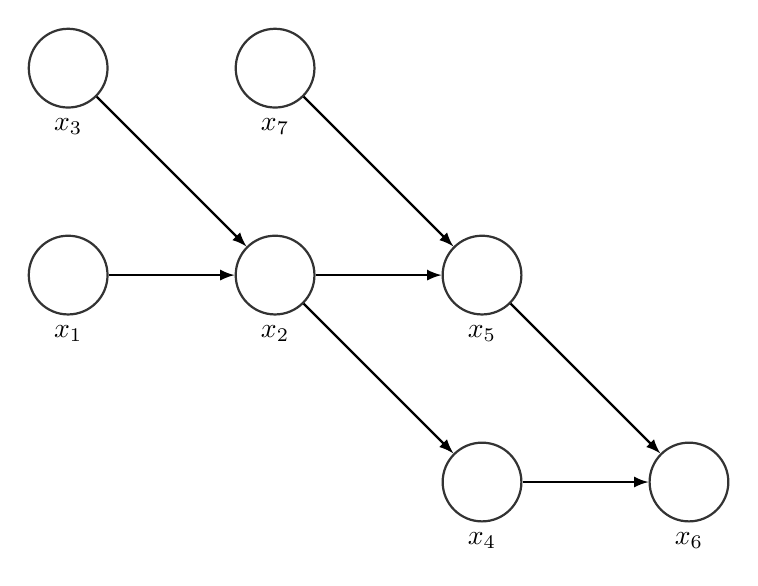
\begin{tikzpicture}
\tikzstyle{main}=[circle, minimum size = 10mm, thick, draw =black!80, node distance = 16mm]
\tikzstyle{connect}=[-latex, thick]
\tikzstyle{box}=[rectangle, draw=black!100]
  \node[main, fill = white!100] (x1) [label=below:$x_1$] { };
  \node[main] (x2) [right=of x1,label=below:$x_2$] { };
  \node[main] (x3) [above=of x1,label=below:$x_3$] {};
  \node[main] (x5) [right=of x2,label=below:$x_5$] { };
  \node[main] (x4) [below=of x5,label=below:$x_4$] { };
  \node[main] (x6) [right=of x4,label=below:$x_6$] { };
  \node[main] (x7) [above=of x2,label=below:$x_7$] { };
  \path (x1) edge [connect] (x2)
           (x3) edge [connect] (x2)
           (x2) edge [connect] (x5)
           (x7) edge [connect] (x5)
           (x2) edge [connect] (x4)
           (x5) edge [connect] (x6)
           (x4) edge [connect] (x6);
\end{tikzpicture}
\end{figure}

The Markov blanket of $x_2$ is $\{x_1, x_3, x_5, x_7 \}$ (the parents, children and co-parents of the children of $x_2$).
\FloatBarrier

\section{}
\textit{Write out the factorization corresponding to the directed graphical model in Figure 10.14a }
\begin{equation} 
\begin{aligned}
Pr(x_1, ..., x_{15}) = &Pr(x_1) Pr(x_2) Pr(x_3) Pr(x_4 | x_1, x_2) Pr(x_5 | x_2, x_3) Pr(x_6) Pr(x_7) Pr(x_8 | x_4, x_5) \\
    & Pr(x_9 | x_3, x_5, x_6) Pr(x_{10} | x_7) Pr(x_{11} | x_8, x_{10}) Pr(x_{12} | x_8, x_9) Pr(x_{13} | x_9) \\
    & Pr(x_{14} | x_{11}) Pr(x_{15} | x_{12}) \notag
\end{aligned} 
\end{equation}

\section{}
\textit{An undirected graphical model has the form}

\begin{equation} 
\begin{aligned}
Pr(x_1, ..., x_{6}) = & \frac{1}{Z} \phi_1[x_1, x_2, x_5] \phi_2[x_2, x_3, x_4] \phi_3[x_1, x_5] \phi_4[x_5, x_6] \notag
\end{aligned} 
\end{equation}

\textit{Draw the undirected graphical model that corresponds to this factorization.}

\begin{figure}[h]
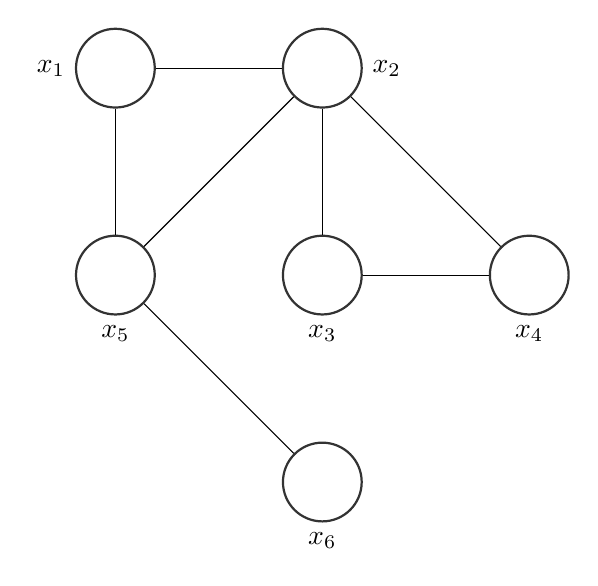
\begin{tikzpicture}
\tikzstyle{main}=[circle, minimum size = 10mm, thick, draw =black!80, node distance = 16mm]
\tikzstyle{connect}=[-latex, thick]
\tikzstyle{box}=[rectangle, draw=black!100]
  \node[main, fill = white!100] (x1) [label=left:$x_1$] { };
  \node[main] (x2) [right=of x1,label=right:$x_2$] { };
  \node[main] (x3) [below=of x2,label=below:$x_3$] {};
  \node[main] (x5) [below=of x1,label=below:$x_5$] { };
  \node[main] (x4) [right=of x3,label=below:$x_4$] { };
  \node[main] (x6) [below=of x3,label=below:$x_6$] { };
  \path (x1) edge (x2)
           (x1) edge (x5)
           (x2) edge (x5)
           (x2) edge (x3)
           (x2) edge (x4)
           (x3) edge (x4)
           (x5) edge (x6)
           ;
\end{tikzpicture}
\end{figure}

\section{}
\textit{Write out the factorization corresponding to the undirected graphical model in Figure 10.14b.}
\begin{equation} 
\begin{aligned}
Pr(x_1, ..., x_{15}) = \frac{1}{Z} &\phi_1[x_3] \phi_2[x_1, x_4] \phi_3[x_2, x_4, x_8] \phi_4[x_2, x_5, x_8] \phi_5[x_5, x_9] \\
  & \phi_6[x_6, x_9] \phi_7[x_8, x_{12}] \phi_8[x_9, x_{12}, x_{13}, x_{15}] \phi_9[x_8, x_{11}] \phi_{10}[x_7, x_{10}] \\
  & \phi_{11}[x_7, x_11] \phi_{12}[x_{11}, x_{14}] \notag
\end{aligned} 
\end{equation}
\FloatBarrier

\section{}
\textit{Consider the undirected graphical model defined over binary values $\{x_i\}_{i=1}^4 \in \{0, 1\}$ defined by }
\begin{equation} 
\begin{aligned}
Pr(x_1, x_2, x_3, x_4) = & \frac{1}{Z} \phi(x_1, x_2) \phi(x_2, x_3) \phi(x_3, x_4) \phi(x_4, x_1) \text{,} \notag
\end{aligned} 
\end{equation}
\textit{where the function $\phi$ is defined by}
\begin{equation} 
\begin{aligned}
&\phi(0,0) = 1 \quad \quad & \phi(1,1) = 2 \\
&\phi(0,1) = 0.1 \quad \quad &\phi(1,0) = 0.1 \notag
\end{aligned} 
\end{equation}
\textit{ Compute the probability of each of the 16 possible states of this system.}

\begin{table}[h]
\begin{tabular}{c c c c|c c c c r r}
\toprule
 $x_1$ & $x_2$ & $x_3$ & $x_4$  & $\phi(x_1, x_2)$ & $\phi(x_2, x_3)$ & $\phi(x_3, x_4)$ & $\phi(x_4, x_1)$ &
       $Z Pr(...)$ & $Pr(...)$ \\ \midrule
 0 & 0 & 0 & 0 & 1. & 1. & 1. & 1. & 1.0000 & .057870 \\
 0 & 0 & 0 & 1 & 1. & 1. & 0.1& 0.1 & 0.0100 & .000579 \\
 0 & 0 & 1 & 0 & 1. & 0.1 & 0.1  & 1. & 0.0100 & .000579 \\
 0 & 0 & 1 & 1 & 1. & 0.1 & 2. & 0.1 & 0.0200 & .001157 \\
 0 & 1 & 0 & 0 & 0.1 & 0.1  & 1. & 1.& 0.0100 & .000579 \\
 0 & 1 & 0 & 1 & 0.1 & 0.1 & 0.1 & 0.1 & 0.0001 & .000006 \\
 0 & 1 & 1 & 0 & 0.1 & 2. & 0.1 & 1. & 0.0200 & .001157 \\
 0 & 1 & 1 & 1 & 0.1 & 2. & 2. & 0.1 & 0.0400 & .002315 \\
 1 & 0 & 0 & 0 & 0.1 & 1. & 1. &  0.1 & 0.0100 & .000579 \\
 1 & 0 & 0 & 1 & 0.1 & 1. & 0.1 & 2. & 0.0200 & .001157 \\
 1 & 0 & 1 & 0 & 0.1 & 0.1 & 0.1 & 0.1 & 0.0001 & .000006 \\
 1 & 0 & 1 & 1 & 0.1 & 0.1 & 2. & 2. & 0.0400 & .002315 \\
 1 & 1 & 0 & 0 & 2.& 0.1 & 1. & 0.1 & 0.0200 & .001157 \\
 1 & 1 & 0 & 1 & 2. & 0.1 & 0.1 & 2. & 0.0400 & .002315 \\
 1 & 1 & 1 & 0 & 2. & 2. & 0.1 & 0.1 & 0.0400 & .002315 \\
 1 & 1 & 1 & 1 & 2. & 2. & 2. & 2. & 16.0000 & .925914 \\ \midrule
 & & & & & & & & 17.2802 & 1.000000 \\ \bottomrule
\end{tabular}
\end{table}
\FloatBarrier 

We can attempt to check this by sampling from the distribution e.g. using Gibbs sampling. To do this we need the conditional probability distribution for each $x_i$. By symmetry we just need to calculate the conditional distribution for $x_1$.

\begin{align*}
  Pr(x_1 | x_{\backslash 1}) &= \frac{Pr(x_1, x_2, x_3, x_4)}{\sum_{x_1} Pr(x_1, x_2, x_3, x_4)} \\
     &= \frac{\frac{1}{Z} \phi(x_1, x_2) \phi(x_2, x_3) \phi(x_3, x_4) \phi(x_4, x_1)}
         {\sum_{x_1}  \frac{1}{Z} \phi(x_1, x_2) \phi(x_2, x_3) \phi(x_3, x_4) \phi(x_4, x_1)} \\
     &= \frac{\phi(x_1, x_2) \phi(x_2, x_3) \phi(x_3, x_4) \phi(x_4, x_1)}
     	{\phi(x_2, x_3) \phi(x_3, x_4) \sum_{x_1} \phi(x_1, x_2) \phi(x_4, x_1)} \\
     &= \frac {\phi(x_1, x_2) \phi(x_4, x_1)}{\sum_{x_1} \phi(x_1, x_2) \phi(x_4, x_1)} \\
 \end{align*}
 \begin{align*}
  Pr(x_1 = 0 | x_2 = 0, x_4 = 0) &= \frac{1. \times 1.}{1. \times 1. + 0.1 \times 0.1} = \frac{1.}{1.01} = 0.9901 \\
  Pr(x_1 = 1 | x_2 = 0, x_4 = 0) &= 1 - Pr(x_1 = 0 | x_2 = 0, x_4 = 0) = 1 - 0.9901 = 0.0099 \\
  Pr(x_1 = 0 | x_2 = 0, x_4 = 1) &= \frac{1. \times 0.1}{1. \times 0.1 + 0.1 \times 2.} = \frac{0.1}{0.3} = 0.3333 \\
  Pr(x_1 = 1 | x_2 = 0, x_4 = 1) &= 1 - Pr(x_1 = 0 | x_2 = 0, x_4 = 0) = 1 - 0.3333 = 0.6667 \\
  Pr(x_1 = 0 | x_2 = 1, x_4 = 0) &= \frac{0.1 \times 1.}{0.1 \times 1. + 2. \times 0.1} = \frac{0.1}{0.3} = 0.3333 \\
  Pr(x_1 = 1 | x_2 = 1, x_4 = 0) &= 1 - Pr(x_1 = 0 | x_2 = 0, x_4 = 0) = 1 - 0.3333 = 0.6667 \\
  Pr(x_1 = 0 | x_2 = 1, x_4 = 1) &= \frac{0.1 \times 0.1}{0.1 \times 0.1 + 2. \times 2.} = \frac{0.01}{4.01} = 0.0025 \\
  Pr(x_1 = 1 | x_2 = 1, x_4 = 1) &= 1 - Pr(x_1 = 0 | x_2 = 0, x_4 = 0) = 1 - 0.0025 = 0.9975 \\
\end{align*}

See problem\_10\_5.py for an implementation.

\section{}
For directed graphical models Markov blanket of a node is the parents, children and co-parents of children of the node. For undirected graphical models Markov blanket of a node is the set of neighbours of that node. Markov blanket, $blanket[]$ for figures 10.7 and 10.8:

\underline{Figure 10.7a}

\begin{flalign*}
blanket[x_1] & \in \{x_3 \} \\
blanket[x_2] & \in \{x_3 \} \\
blanket[x_3] & \in \{x_1, x_2 \}
\end{flalign*}

\underline{Figure 10.7b}

\begin{flalign*}
blanket[x_1] & \in \{x_3 \} \\
blanket[x_2] & \in \{x_3 \} \\
blanket[x_3] & \in \{x_1, x_2 \}
\end{flalign*}

\underline{Figure 10.7c}

\begin{flalign*}
blanket[x_1] & \in \{x_2, x_3 \} \\
blanket[x_2] & \in \{x_1, x_3 \} \\
blanket[x_3] & \in \{x_1, x_2 \}
\end{flalign*}

\underline{Figure 10.8a}

\begin{flalign*}
blanket[x_1] & \in \{x_2, x_3 \} \\
blanket[x_2] & \in \{x_1, x_4 \} \\
blanket[x_3] & \in \{ x_1, x_4 \} \\
blanket[x_4] & \in \{x_2, x_3 \}
\end{flalign*}

\underline{Figure 10.8b}

\begin{flalign*}
blanket[x_1] & \in \{x_2, x_3 \} \\
blanket[x_2] & \in \{x_1, x_3, x_4 \} \\
blanket[x_3] & \in \{ x_1, x_2, x_4 \} \\
blanket[x_4] & \in \{x_2, x_3 \}
\end{flalign*}

\section{}
\textit{Show that the stated patterns of independence and conditional independence in Figures 10.7 and 10.8 are true.}

For Figure 10.7a we need to prove that $x_2 \independent x_1 | x_3$. We use the same strategy as given in the text in "10.2.2 Example 1". We write down the conditional probability statement for $x_2$ \textit{including $x_1$}, the variable we are trying to show $x_2$ is conditionally independent of. Then we show by algebraic manipulation that there is a representation of the conditional probability that does not include $x_1$

\begin{align*}
Pr(x_2 | x_1, x_3) & = \frac{Pr(x_1, x_2, x_3)}{Pr(x_1, x_3)} \\
   & = \frac{Pr(x_2 | x_3) Pr(x_3 | x_1) Pr(x_1)}{\int Pr(x_2 | x_3) Pr(x_3 | x_1) Pr(x_1) dx_2} \\
   & = \frac{Pr(x_2 | x_3) Pr(x_3 | x_1) Pr(x_1)}{Pr(x_3 | x_1) Pr(x_1) \int Pr(x_2 | x_3)  dx_2} \\
   & = \frac{Pr(x_2| x_3)}{\int Pr(x_2 | x_3)  dx_2}
\end{align*}
The final expression doesn't depend on $x_1$ so we conclude that the conditional independence statement holds.

For Figure 10.7b this is just the same argument as in "10.3.1. Example 1" of the text but with a relabelling of the graph.

For Figure 10.7c we prove the (unconditional) independence statement $x_2 \independent x_1$ by showing that $Pr(x_2, x_1) = Pr(x_2) Pr(x_1)$

\begin{align*}
Pr(x_2,  x_1) & = \int Pr(x_2, x_1, x_3) dx_3 \\
   & = \int Pr(x_2) Pr(x_1) Pr(x_3 | x_1, x_2) dx_3 \\
   & = Pr(x_2) Pr(x_1) \int Pr(x_3 | x_1, x_2) dx_3 \\
   & = Pr(x_2) Pr(x_1)
\end{align*}
where the last step uses the fact that $\int Pr(x_3 | x_1, x_2) dx_3  = 1$.

For Figure 10.8a we again write down the conditional probability statement including the variables we wish to show are (conditionally independent)

\begin{align*}
Pr(x_1 | x_4, x_2, x_3) & = \frac{Pr(x_1, x_4, x_2, x_3)}{Pr(x_4, x_2, x_3)} \\
   & = \frac{\frac{1}{Z} \phi_1(x_1, x_2) \phi_2(x_2, x_4) \phi_3(x_4, x_3) \phi_4(x_3, x_1)}
            {\int \frac{1}{Z} \phi_1(x_1, x_2) \phi_2(x_2, x_4) \phi_3(x_4, x_3) \phi_4(x_3, x_1) dx_1} \\
   & = \frac{\frac{1}{Z} \phi_1(x_1, x_2) \phi_2(x_2, x_4) \phi_3(x_4, x_3) \phi_4(x_3, x_1)}
            {\frac{1}{Z} \phi_2(x_2, x_4) \phi_3(x_4, x_3) \int  \phi_1(x_1, x_2)  \phi_4(x_3, x_1) dx_1} \\
   & = \frac{ \phi_1(x_1, x_2)  \phi_4(x_3, x_1)}
            { \int \phi_1(x_1, x_2)  \phi_4(x_3, x_1) dx_1} \\
\end{align*}
and the final expression does not rely on $x_4$

The proof of $x_2 \independent x_3 | x_1, x_4$ is similar:

\begin{align*}
Pr(x_2 | x_3, x_1, x_4) & = \frac{Pr(x_1, x_4, x_2, x_3)}{Pr(x_1, x_3, x_4)} \\
   & = \frac{\frac{1}{Z} \phi_1(x_1, x_2) \phi_2(x_2, x_4) \phi_3(x_4, x_3) \phi_4(x_3, x_1)}
            {\int \frac{1}{Z} \phi_1(x_1, x_2) \phi_2(x_2, x_4) \phi_3(x_4, x_3) \phi_4(x_3, x_1) dx_2} \\
   & = \frac{\frac{1}{Z} \phi_1(x_1, x_2) \phi_2(x_2, x_4) \phi_3(x_4, x_3) \phi_4(x_3, x_1)}
            {\frac{1}{Z}  \phi_3(x_4, x_3) \phi_4(x_3, x_1)\int \phi_1(x_1, x_2) \phi_2(x_2, x_4)  dx_2} \\
   & = \frac{ \phi_1(x_1, x_2) \phi_2(x_2, x_4)}
            {\int \phi_1(x_1, x_2) \phi_2(x_2, x_4)  dx_2} \\
            & \implies x_2 \independent x_3 | x_1, x_4
\end{align*}

For figure 10.8b let's prove the first assertion using the (by now) familiar technique

\begin{align*}
Pr(x_1 | x_4, x_2, x_3) & = \frac{Pr(x_1, x_4, x_2, x_3)}{Pr(x_4, x_2, x_3)} \\
    & = \frac{Pr(x_1) Pr(x_2 | x_1) Pr(x_3 | x_1) Pr(x_4 | x_2, x_3)}{\int  Pr(x_1) Pr(x_2 | x_1) Pr(x_3 | x_1) Pr(x_4 | x_2, x_3) dx_1} \\
    & =  \frac{Pr(x_1) Pr(x_2 | x_1) Pr(x_3 | x_1) Pr(x_4 | x_2, x_3)}{Pr(x_4 | x_2, x_3) \int  Pr(x_1) Pr(x_2 | x_1) Pr(x_3 | x_1)  dx_1} \\
    & =  \frac{Pr(x_1) Pr(x_2 | x_1) Pr(x_3 | x_1) }{\int  Pr(x_1) Pr(x_2 | x_1) Pr(x_3 | x_1)  dx_1} \\
    & \implies x_1 \independent x_4 | x_2, x_3
\end{align*}

and then the 2nd assertion

\begin{align*}
Pr(x_2 | x_3, x_1) & = \frac{Pr(x_2, x_3, x_1)}{Pr(x_3, x_1)} \\
    & = \frac{\int Pr(x_2, x_3, x_1, x_4) dx_4}{\int \int Pr(x_2, x_3, x_1, x_4) dx_4 dx_2} \\
    & = \frac{\int Pr(x_1) Pr(x_2 | x_1) Pr(x_3 | x_1) Pr(x_4 | x_2, x_3) dx_4}
                 {\int \int Pr(x_1) Pr(x_2 | x_1) Pr(x_3 | x_1) Pr(x_4 | x_2, x_3)  dx_4 dx_2} \\
    & = \frac{Pr(x_1) Pr(x_2 | x_1) Pr(x_3 | x_1) \int  Pr(x_4 | x_2, x_3) dx_4}
                 {Pr(x_1) Pr(x_3 | x_1) \int  Pr(x_2 | x_1) \int Pr(x_4 | x_2, x_3)  dx_4 dx_2} \\
    & = \frac{Pr(x_2 | x_1) \int  Pr(x_4 | x_2, x_3) dx_4}
                 { \int  Pr(x_2 | x_1) \int Pr(x_4 | x_2, x_3)  dx_4 dx_2} \\
    & = \frac{Pr(x_2 | x_1) }{ \int  Pr(x_2 | x_1)  dx_2} \\
    & = Pr(x_2 | x_1)
\end{align*}


\section{}
\textit{Draw the factor graphs corresponding to the graphical models in Figures 10.7 and 10.8. You must first establish the factorized joint distribution associated with each graph.}

\begin{figure}[h]
\center
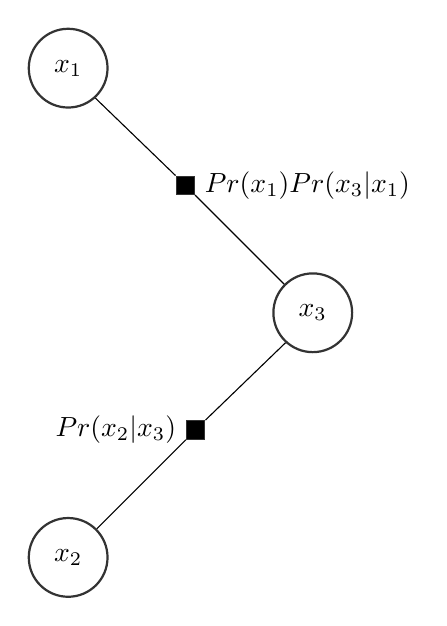
\begin{tikzpicture}
\tikzstyle{main}=[circle, minimum size = 10mm, thick, draw =black!80, node distance = 16mm]
\tikzstyle{factor}=[rectangle, draw =black!80, fill = black!100]
\tikzstyle{connect}=[-latex, thick]
\tikzstyle{box}=[rectangle, draw=black!100]
  \node[main, fill = white!100] (x1)  { $x_1$ };
\node[factor] (f1) [below right =of x1,label=right:$Pr(x_1)Pr(x_3|x_1)$] { };
  \node[main] (x3) [below right =of f1] { $x_3$ };
\node[factor] (f2) [below left =of x3,label=left:$Pr(x_2 | x_3)$] { };
  \node[main] (x2) [below left =of f2] { $x_2$ };
  \path (x1) edge (f1)
           (f1) edge (x3)
           (x3) edge (f2)
           (f2) edge (x2)
           ;
\end{tikzpicture}
\caption*{Figure 10.7a}
\end{figure}

\begin{figure}[h]
\center
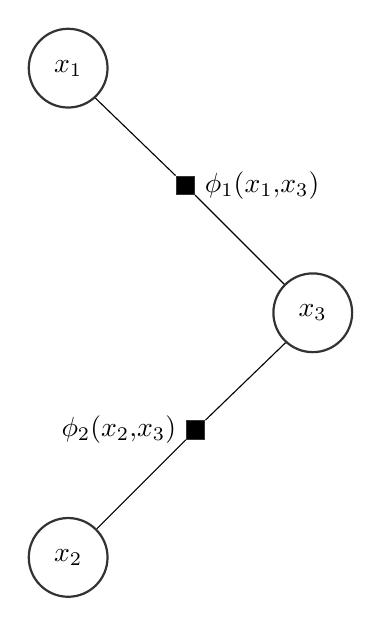
\begin{tikzpicture}
\tikzstyle{main}=[circle, minimum size = 10mm, thick, draw =black!80, node distance = 16mm]
\tikzstyle{factor}=[rectangle, draw =black!80, fill = black!100]
\tikzstyle{connect}=[-latex, thick]
\tikzstyle{box}=[rectangle, draw=black!100]
  \node[main, fill = white!100] (x1)  { $x_1$ };
\node[factor] (f1) [below right =of x1,label=right:$\phi_1(x_1{,} x_3)$] { };
  \node[main] (x3) [below right =of f1] { $x_3$ };
\node[factor] (f2) [below left =of x3,label=left:$\phi_2(x_2 {,} x_3)$] { };
  \node[main] (x2) [below left =of f2] { $x_2$ };
  \path (x1) edge (f1)
           (f1) edge (x3)
           (x3) edge (f2)
           (f2) edge (x2)
           ;
\end{tikzpicture}
\caption*{Figure 10.7b}
\end{figure}
\FloatBarrier

The third graph is a little more tricky. The factorization is $Pr(x_1, x_2, x_3) = Pr(x_1) Pr(x_2) Pr(x_3 | x_1, x_2)$. There is no 'nice' way to split the 3rd term so we need to create a 3-way factor.
\begin{figure}[h]
\center
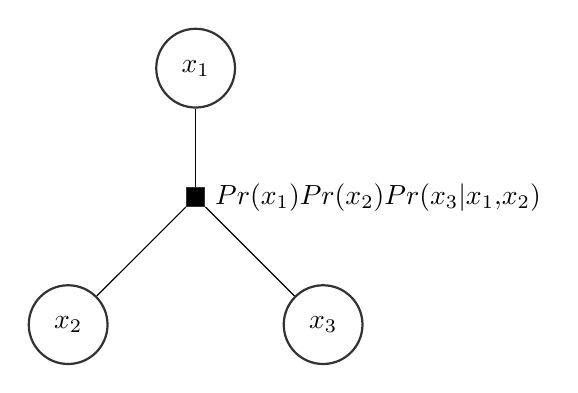
\begin{tikzpicture}
\tikzstyle{main}=[circle, minimum size = 10mm, thick, draw =black!80, node distance = 16mm]
\tikzstyle{factor}=[rectangle, draw =black!80, fill = black!100]
\tikzstyle{connect}=[-latex, thick]
\tikzstyle{box}=[rectangle, draw=black!100]
  \node[main, fill = white!100] (x1)  { $x_1$ };
\node[factor] (f1) [below  =of x1,label=right:$Pr(x_1) Pr(x_2) Pr(x_3 | x_1{,} x_2)$] { };
  \node[main] (x3) [below right =of f1] { $x_3$ };
  \node[main] (x2) [below left =of f1] { $x_2$ };
  \path (x1) edge (f1)
           (f1) edge (x3)
           (f1) edge (x2)
           ;
\end{tikzpicture}
\caption*{Figure 10.7c}
\end{figure}

\begin{figure}[h]
\center
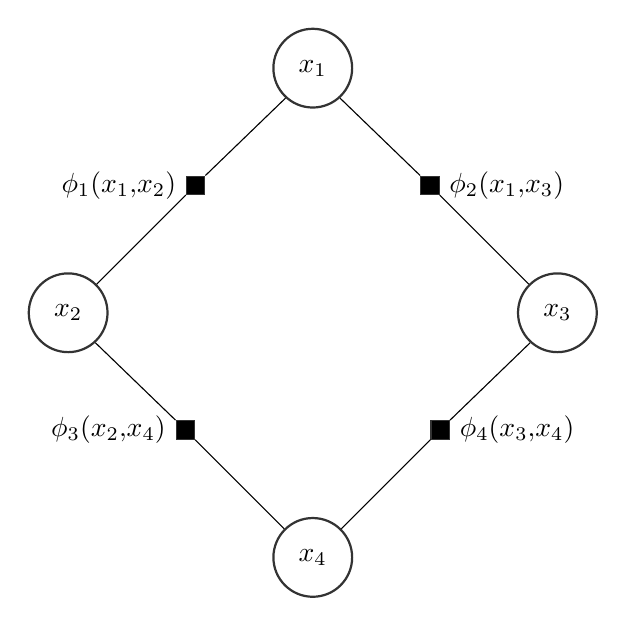
\begin{tikzpicture}
\tikzstyle{main}=[circle, minimum size = 10mm, thick, draw =black!80, node distance = 16mm]
\tikzstyle{factor}=[rectangle, draw =black!80, fill = black!100]
\tikzstyle{connect}=[-latex, thick]
\tikzstyle{box}=[rectangle, draw=black!100]
  \node[main, fill = white!100] (x1)  { $x_1$ };
\node[factor] (f1) [below left =of x1,label=left:$\phi_1(x_1{,} x_2)$] { };
  \node[main] (x2) [below left =of f1] { $x_2$ };
  \node[factor] (f2) [below right =of x1,label=right:$\phi_2(x_1{,}x_3)$] { };
  \node[main] (x3) [below right =of f2] { $x_3$ };
  \node[factor] (f3) [below right =of x2,label=left:$\phi_3(x_2 {,} x_4)$] { };
  \node[factor] (f4) [below left =of x3,label=right:$\phi_4(x_3 {,} x_4)$] { };
  \node[main] (x4) [below right =of f3] { $x_4$ };
\path (x1) edge (f1)
           (f1) edge (x2)
           (x1) edge (f2)
           (f2) edge (x3)
           (x2) edge (f3)
           (x3) edge (f4)
           (f3) edge (x4)
           (f4) edge (x4)
           ;
\end{tikzpicture}
\caption*{Figure 10.8a}
\end{figure}
\FloatBarrier

Again it's helpful to write out the full joint probability $Pr(x_1, x_2, x_3, x_4) = Pr(x_1) Pr(x_2 | x_1) Pr(x_3, x_1) Pr(x_4 | x_2, x_3)$. Once more the last term forces us to have a 3-way factor node. Also we now have options of where to put $Pr(x_1)$. We can put it in the factor node for $x_1, x_2$ or in the node for $x_1, x_3$ or we could simply have a a single node for $Pr(x_1)$ hanging off $x_1$. Here I have decided on the first option.

\begin{figure}[h]
\center
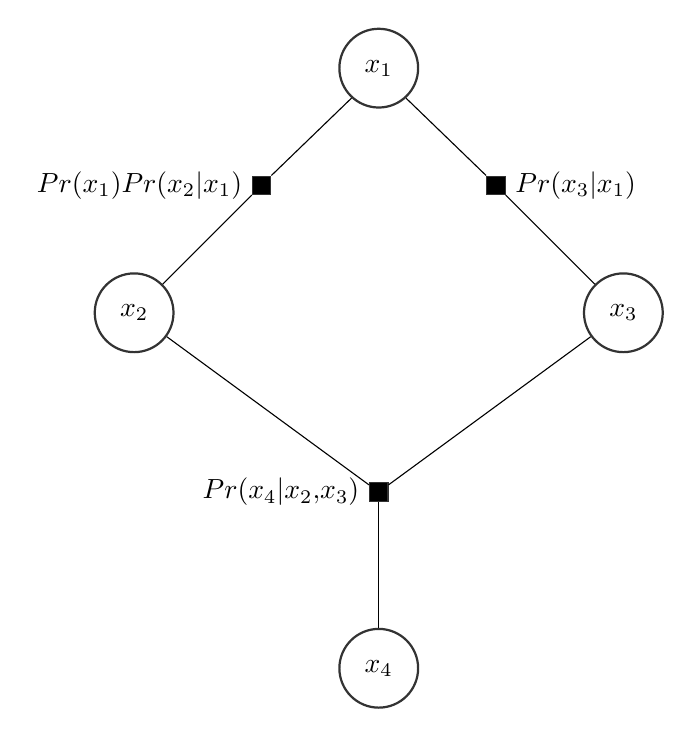
\begin{tikzpicture}
\tikzstyle{main}=[circle, minimum size = 10mm, thick, draw =black!80, node distance = 16mm]
\tikzstyle{factor}=[rectangle, draw =black!80, fill = black!100]
\tikzstyle{connect}=[-latex, thick]
\tikzstyle{box}=[rectangle, draw=black!100]
  \node[main, fill = white!100] (x1)  { $x_1$ };
  \node[factor, draw =white!80, fill = white!100] (x1a) [below =of x1, label=] {};
  \node[factor, draw =white!80, fill = white!100] (x1b) [below =of x1a, label=] {};
  \node[factor, draw =white!80, fill = white!100] (x1c) [below =of x1b, label=] {};
\node[factor] (f1) [below left =of x1,label=left:$Pr(x_1) Pr(x_2 | x_1)$] { };
  \node[main] (x2) [below left =of f1] { $x_2$ };
  \node[factor] (f2) [below right =of x1,label=right:$Pr(x_3 | x_1)$] { };
  \node[main] (x3) [below right =of f2] { $x_3$ };
  \node[factor] (f3) [below =of x1c,label=left:$Pr(x_4 | x_2 {,} x_3)$] { };
  \node[main] (x4) [below =of f3] { $x_4$ };
\path (x1) edge (f1)
           (f1) edge (x2)
           (x1) edge (f2)
           (f2) edge (x3)
           (x2) edge (f3)
           (x3) edge (f3)
           (f3) edge (x4)
           ;
\end{tikzpicture}
\caption*{Figure 10.8a}
\end{figure}

\section{}
\textit{What is the Markov blanket of variable $w_2$ in Figure 10.9c?}


\begin{flalign*}
blanket[w_2] & = \{w_1, w_5, x_2, w_4\}
\end{flalign*}


\section{}
\textit{What is the Markov blanket of variable $w_8$ in Figure 10.9e?}

We have to combine the definitions of Markov blanket for directed and undirected graphical models. The only directed child, parent or parent-of-child for $w_8$ is $x_8$. The undirected neighbours of $w_8$ are $w_5, w_7, w_9, w_11$. 

\begin{flalign*}
blanket[w_8] & = \{x_8, w_5, w_7, w_9, w_11\}
\end{flalign*}


\end{document}